\documentclass[11pt]{article}
\usepackage[utf8]{inputenc}
\usepackage[T1]{fontenc}
\usepackage{amsmath}
\usepackage{amsfonts}
\usepackage{amssymb}
\usepackage[version=4]{mhchem}
\usepackage{stmaryrd}
\usepackage{graphicx}
\usepackage[export]{adjustbox}
\graphicspath{ {./images/} }

\begin{document}
The Term Structure of Forward Prices on Commodities

Session 2.6, Derivatives and Risk-Neutral Valuation, focuses on the term structure of forward contracts with financial securities as their underlying asset. The slope and shape of the forward curve for these financial contracts is shown in that session through an arbitrage-free model (the cost-of-carry model) to depend on only two factors: market (riskless) interest rates and the distribution rate (e.g., divided yield) of the underlying asset. This lesson discusses the term structure of forward prices on commodities. The slope and shape of the forward curve for certain commodities were shown in the Derivatives and Risk-Neutral Valuation session to depend on three factors: market interest rates, storage costs, and convenience yield. This session includes the effects of anticipated changes in supply and demand, in particular the supply effects of harvests.

\section*{Costs of Carry for Commodities}
The Derivatives and Risk-Neutral Valuation session discusses the costs of carrying physical inventories as important inputs to the pricing of forward contracts on commodities. The forward price of a commodity, $F_{T}$, is found based on carrying costs and the spot price of the commodity, $P_{0}$, as depicted in Equation 1 and reproduced below:


\begin{equation*}
F_{T} \leq P_{0} e^{(r+c-y) T} \tag{1}
\end{equation*}


\begin{center}
\begin{tabular}{|lcc|}
\hline
\multicolumn{3}{c|}{Cost of Carry} \\
\hline
Cost of Carry & Per Month & Three Months \\
\hline
Spot price per bushel &  & $\$ 4.25$ \\
Financing rate & $0.20 \%$ & $\$ 0.026$ \\
Spoilage rate & $0.165 \%$ & $\$ 0.021$ \\
Convenience yield & $0.20 \%$ & $-\$ 0.026$ \\
Storage cost per bushel & $\$ 0.010$ & $\$ 0.030$ \\
Total cost of carry &  & $\$ 0.051$ \\
Break-even futures price &  & $\$ 4.301$ \\
\hline
\end{tabular}
\end{center}

where $r$ is the spot (riskless) interest rate corresponding to a time-to-maturity of $T$ years, $c$ is the commodity's storage cost, and $y$ is the commodity's convenience yields, all expressed as continuously compounded annual rates. Cost-of-carry models assume that in an informationally efficient market, when two positions converge to an equivalent value at some point in the future, any differences in their current prices will be determined exactly by the differences in their carrying costs.

In addition to the costs of carry introduced in the Derivatives and Risk-Neutral Valuation session, in some cases other carrying costs are included. For example, in the case of perishable commodities, spoilage costs may be modeled separately as a cost of carry or may be included as a storage cost. Spoilage cost is the loss of value that may naturally occur through time during storage due to physical deterioration. Inventory shrinkage is loss of inventory through time due to theft, decline in moisture content, and so forth.

The above exhibit displays an example of the cost of carry. In this case, the spot price per bushel of corn is $\$ 4.25$. For simplification, the costs of carry are assumed to be payable at the end of the carry period (three months). Given the components of the cost of carry presented in the exhibit, one would be indifferent when choosing between purchasing the corn in the spot market for $\$ 4.25$ and carrying the commodity for three months, and purchasing the corn in the futures market for $\$ 4.301$ and taking delivery in three months.

As noted in the previous equation, the cost-of-carry model indicates a maximum forward price. When arbitrageurs cannot borrow a commodity without incurring expenses (other than the time value of money), it is possible that forward prices will be less than those implied by the cost-of-carry model. Two clear examples would be the forward price of a grain deliverable after the next harvest or the forward price of natural gas after the winter heating season. When there is a convenience yield, $y$, forward prices tend to be less than those implied by the cost-of-carry model. Therefore, the futures price of $\$ 4.301$ is a maximum price above which arbitrage would be possible and below which arbitrage may or may not be possible based on convenience yield and the ability to short-sell the commodity.

\section*{Harvests, Supply Elasticity, and Shifts in Demand}
A key issue in understanding the term structure of forward prices is the rate at which and the extent to which changes in the supply and demand of a commodity can be predicted. Those predictions (such as a bumper crop of grain after several years of drought) can substantially influence the shape of the forward price curve of the commodity.

With regard to supply, on one end of the spectrum is a perfectly elastic supply. Perfectly elastic supply describes a market in which any quantity demanded can be instantaneously and limitlessly supplied without changes in the market price, and is associated with little or no convenience yield. Currencies provide an example of an item with a supply that can be changed rapidly (in this case, by a central bank).

On the other end of the spectrum are commodities with inelastic supply. Inelastic supply is when supplies of the item change slowly in response to market prices or when large changes in market prices are necessary to effect supply changes, and is associated with high convenience yield. An example of sluggishly responding supply is an agricultural commodity that is harvested annually. At any particular point in time, not only is additional supply not available until the next harvest, but the size of the next harvest may have already been determined by such decisions as the acreage planted. When the supply of a commodity cannot respond quickly to meet changing demand, it is likely that its convenience yield will be higher, since users of the commodity may have greater fear of shortages.

Demand for commodities can shift, based on factors such as levels of economic activity and consumer preferences. Demand for some goods, such as grain, may shift slowly or moderately as needs for livestock feed shift. The demand for other goods, such as natural gas, may change more rapidly due to factors such as weather. When demand can change quickly, the convenience yield is likely to be higher, since users of the commodity may have greater fear of shortages. Inelastic demand is a market condition in which the demand for a good does not increase or decrease substantially due to changes in price and therefore is a potential cause of higher price volatility and higher convenience yield.

Forecasts of supply and demand shifts can affect not only the current price level of a commodity but also the slope and shape of the term structure of forward prices. These potential complexities add to both the threats and the opportunities for commodities traders and managers of managed futures programs. The challenges can be addressed with both fundamental and technical analysis, with those performing and implementing superior analysis earning better returns than those performing and implementing poor analysis.

\section*{Backwardation and Contango}
The slope of the term structure of futures and forward contracts on financial assets is discussed in Session 2.6, Derivatives and Risk-Neutral Valuation. The term structure (i.e., futures or forward curve) is formed as the relation between delivery dates and price (or rates in the case of contracts on rates). In the case of futures contracts, the possible delivery (settlement) dates are determined by the exchange on which the futures are traded and are typically spaced in weeks, months, or quarters. Forward contract settlement dates are usually negotiated between the parties and can therefore occur on virtually any trading day.

The exhibit Term Structure of Forward Prices: Contango, Flat, and Backwardation illustrates the possible slopes of the term structure of forward prices on commodities along with the terms for those slopes in the study of commodities.

When the term structure of forward prices is upward sloping (i.e., when more distant forward contracts have higher prices than contracts that are nearby), the market is said to be in contango. Contango also refers to a forward price exceeding the current spot price (viewing a spot price as a forward price with zero time to delivery may provide clarity). When the slope of the term structure of forward prices is negative, the market is in backwardation, or is backwardated. The concept of backwardation is the complement to contango.

\begin{center}
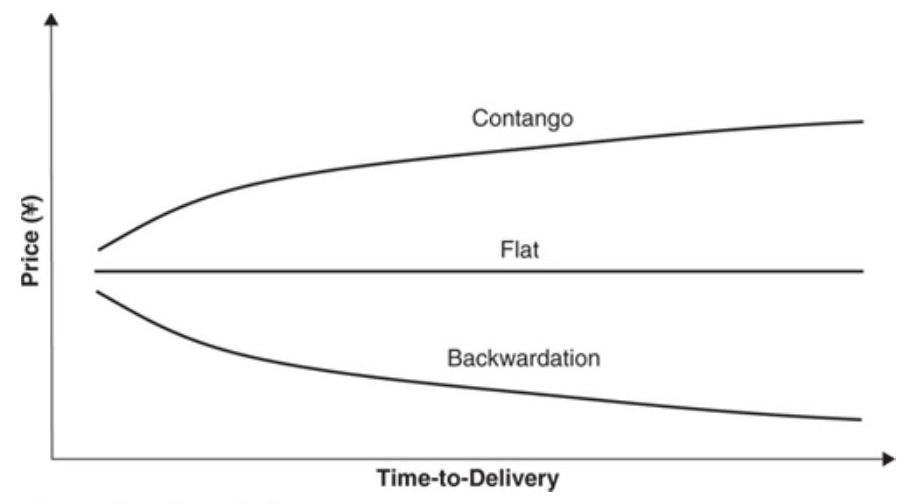
\includegraphics[max width=\textwidth]{2024_04_11_00d1b46832d5f98705cdg-3}
\end{center}

Term Structure of Forward Prices: Contango, Flat, and Backwardation

Recall from the Derivatives and Risk-Neutral Valuation session that the term structure of forward prices on financial securities is upward sloping (i.e., in contango) when the riskless rate exceeds the underlying asset's dividend yield. In rare cases, the slope may be downward (i.e., in backwardation) if the dividend yield on the deliverable (underlier) exceeds the risk-free rate.

\section*{How Backwardation and Contango Reflect Cost of Carry in a Perfect Market}
The Derivatives and Risk-Neutral Valuation session demonstrated that in the case of forward contracts on financial assets, the slope of the term structure of forward prices was driven entirely by the two costs of carry: interest rates and dividends (the benefits of dividends are included as a negative cost). A critical assumption was that of perfect financial markets in which there are no transactions costs, or restrictions on transactions-especially short-selling.

In a perfect and informationally efficient market for financial assets, contango and backwardation occur to prevent arbitrage opportunities that would otherwise exist if the term structure of forward contracts on financial assets were flat when the riskless rate differed from the dividend yield.

A close look at the determination of financial forward prices illustrates two important points: (1) backwardation, contango, and, in fact, the entire slope and shape of the term structure are determined by differences in cost of carry, and (2) in an efficient market, all forward contracts offer equal risk-adjusted expected returns, regardless of the slope and shape of the term structure of forward prices.

\section*{Backwardation and Contango in an Imperfect Market}
Three major issues inhibit the arbitrage activity that ensures the relation between carrying costs and the shape of forward curves discussed in the previous section.

First, unlike the cost of carry to a financial security (the cost of financing), the storage costs of commodities can vary substantially through time and among market participants. The supply of physical storage facilities is inelastic, meaning that changes in demand for storage can dramatically affect marginal storage costs. The exhibit Term Structure of Natural Gas Futures Closing Prices from the lesson Forward Contracts on Assets with Benefits and Costs of Carry in Session 2.6, Derivatives and Risk-Neutral Valuation, indicated the effects of predictable demand patterns on forward natural gas prices in the presence of storage constraints.

Second, unlike the benefit of carry to a financial security (dividends and other distributions), the convenience yield to commodities can vary substantially through time and among market participants. The marginal benefits of holding inventories can change dramatically based on current and anticipated inventory levels. The exhibit Corn Futures Prices indicates the effects of predictable supply patterns (i.e., harvests) on forward corn prices in the presence of demand inelasticity, where the July futures tend to be higher than in other expiration months.

Finally, difficulties in borrowing commodities-especially those that are in short supply-inhibit the ability of arbitrageurs to short-sell such that forward prices are driven to levels based on the cost-of-carry model, including convenience yield.

As a result, the slope of the forward curves for commodities (backwardation vs. contango), as well as the shape, is driven by complex factors. Understanding the complex dynamics of commodity forward prices is a challenge with substantial potential benefits to those market participants with superior knowledge or skill. Commodities that have tremendous variations in demand (e.g., natural gas across winter vs. summer in the northern hemisphere) and variations in supply (grains across growing seasons) lead to price changes that in turn lead to challenges and opportunities for investors and speculators.

\begin{center}
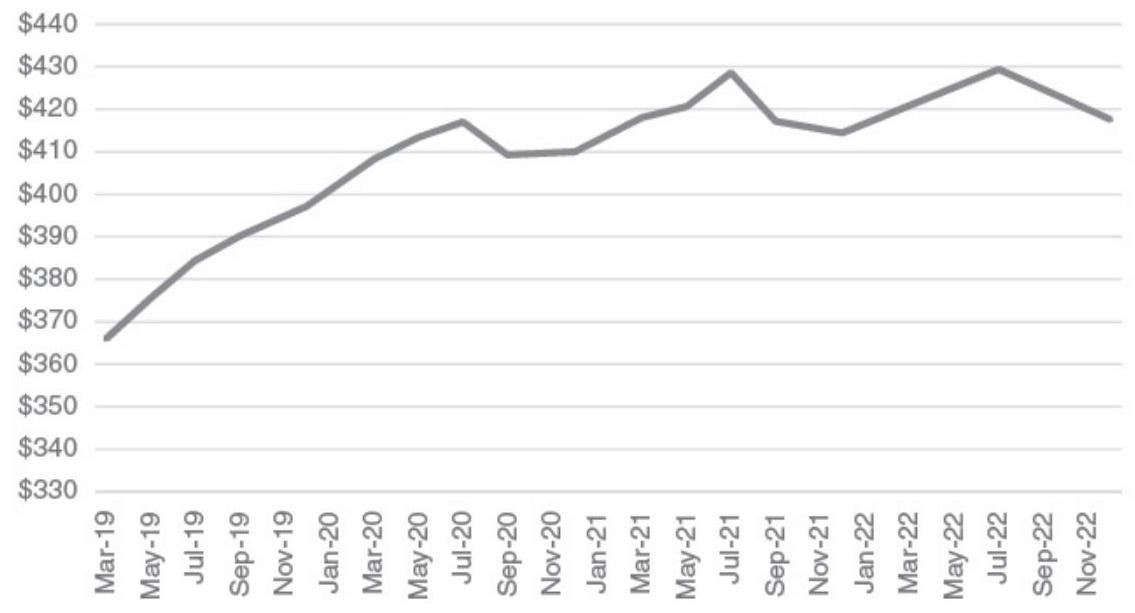
\includegraphics[max width=\textwidth]{2024_04_11_00d1b46832d5f98705cdg-4}
\end{center}

Corn Futures Prices

\section*{The Basis of Forward and Futures Contracts}
The basis of futures or forward contracts is commonly defined as the spot price minus the futures or forward price, although in some literature the basis is defined as the forward price minus the spot price. Basis risk is the dispersion in economic returns associated with changes in the relation between spot prices and futures prices. The basis of a forward contract with delivery in $T$ years, $F_{T}$, on a referenced asset with price, $S$, is depicted in Equation 2:


\begin{equation*}
\text { Basis }=S-F_{T} \tag{2}
\end{equation*}


Again, in some sources the basis is defined as the forward price minus the spot price. The basis is equal to the present value of the carrying costs (perhaps multiplied by -1 , depending on the definition used). Note that at delivery (i.e., time $T$ ) $S=F_{T}$ (i.e., the prices converge at delivery, since a forward contract with zero time to delivery is a spot transaction). Analysts study the behavior of the basis through time, recognizing convergence. Convergence, previously defined as the spot price approaching the forward price as delivery approaches, can also be viewed as the basis approaching zero as the time of delivery approaches.

An arbitrageur or trader hedging spot positions against forward positions analyzes the basis, compares it to carrying costs, and attempts to identify mispricing. To the extent that markets are informationally efficient, a position that is short the forward contract and long the spot price is hedged and should offer an expected return equal to the cost of carry (before transaction costs). The opposite position (long the futures and short the spot) is, in effect, borrowing money by selling or short selling an asset. That trade is also riskless and generates a borrowing cost equal to the carrying costs.

\section*{Calendar Spreads on Forward Contracts}
Traders hedging forward contracts against each other focus on the calendar spread between the prices of the contracts, as depicted in Equation 3:

Calendar Spread $=F_{T+t}-F_{T}$

where $t$ is the length of time separating the settlement dates of the contracts. A calendar spread can be viewed as the difference between futures prices (or forward prices) on the same underlying asset but with different settlement dates. A calendar spread can also be viewed as a position: the simultaneous long and short positions in forward contracts with the same underlying commodity but with different times to delivery. Thus, the trader may calculate the calendar spread as a numerical concept, and may put on a calendar spread by taking hedged positions in the contracts. Other types of spreads may be formed based on distinctions between contracts other than settlement dates.

Calendar spread trading focuses on the search for relatively mispriced futures or forward contracts on the same commodity but with different settlement dates. Calendar spread trading is therefore a speculation on changes in the shape and slope of the term structure of forward prices.

\section*{The Return on a Calendar Spread}
The return on a calendar spread (ignoring dividends, which are common in financial futures) must depend on the same variables that determine forward prices, which in Equation 2 are the spot price $(S)$, the riskless financing rate $(r)$, the storage costs $(c)$, and the convenience yield $(y)$.

Note that in the previous example, the trader had equally sized long and short positions. In this unique situation of a level-term structure of forward contracts, a trader can have the same notional value in each position by having the same number of contracts. If the term structure of forward prices has a slope, then the notional value of each contract differs, and a trader with offsetting positions with equal numbers of contracts will not be hedged in terms of notional values.

In summary, calendar spreads that contain long and short positions of equal notional value are hedged against changes in the spot price. Changes in the spot price (everything else being equal) may be viewed as causing a parallel or additive shift in the entire term structure of forward prices. Changes in the costs of carry cause a slope change in the term structure of forward prices. Returns on calendar spreads are primarily driven by two equivalent concepts: changes in the slope of the term structure of forward prices, and changes in carrying costs.

\section*{The Risks of a Calendar Spread}
Individual positions in forward contracts are quite sensitive to the price of the underlying asset. But as illustrated in the previous section The Return on a Calendar Spread, a calendar spread based on notional values may have little or no sensitivity to the price of the underlying asset.

Note from Equation 2 in the lesson Forward Contracts on Assets with Benefits and Costs of Carry in Session 2.6 that the sensitivity of the price of a forward contract with respect to the carrying costs is proportional to the time to settlement of the contract $(t)$. This leads to two properties regarding the risks of calendar spreads:

\begin{enumerate}
  \item The value of a calendar spread is sensitive to carrying costs. The degree of sensitivity that a calendar spread has to carry costs is driven by the amount of time that separates the times to settlement of the contracts that form the spread. Thus, spreads with underlying contracts that differ more in longevity tend to be riskier.

  \item Spreads that are long the longer-term contract benefit when costs of carry rise, and suffer when costs of carry decline. The intuition is that the benefit of a forward contract is avoiding the costs of carrying a cash position in an asset. When carrying costs rise, longer-term forward contracts enjoy a larger increase in total benefits than is enjoyed by shorter-term contracts.

\end{enumerate}

The concept that longer-term forward contracts are positively related to carrying costs and more sensitive than shorter-term contracts can be confirmed by noting that the partial derivative of $F(T)$ in Equation 2 in the lesson Forward Contracts on Assets with Benefits and Costs of Carry with respect to carrying costs ( $r$ and $c$ ) is $T$ $F(T)$.


\end{document}